%%%%%%%%%%%%%%%%%%%%%%%%%%%%%%%%%%%%%%%%%%%%%%%%%%%%%%%%%%%%%%%%%%%%%%
% How to use writeLaTeX: 
%
% You edit the source code here on the left, and the preview on the
% right shows you the result within a few seconds.
%
% Bookmark this page and share the URL with your co-authors. They can
% edit at the same time!
%
% You can upload figures, bibliographies, custom classes and
% styles using the files menu.
%
%%%%%%%%%%%%%%%%%%%%%%%%%%%%%%%%%%%%%%%%%%%%%%%%%%%%%%%%%%%%%%%%%%%%%%

\documentclass[12pt]{article}

\usepackage{sbc-template}

\usepackage{graphicx,url}

%\usepackage[brazil]{babel}   
\usepackage[utf8]{inputenc}  

     
\sloppy

\title{Nome do artigo}

\author{Roberto N. Mourão\inst{1}, Filipe G. de O. Almeida\inst{1}, Igor T. V. Stemler\inst{1} }


\address{Departamento de Ciência da Computação -- Universidade de Brasília
  (UnB)\\
  \email{\{nedel,flavio\}@inf.ufrgs.br, filipegoa@gmail.com,
  jomi@inf.furb.br}
}

\begin{document} 

\maketitle

\begin{abstract}
  This meta-paper describes the style to be used in articles and short papers
  for SBC conferences. For papers in English, you should add just an abstract
  while for the papers in Portuguese, we also ask for an abstract in
  Portuguese (``resumo''). In both cases, abstracts should not have more than
  10 lines and must be in the first page of the paper.
\end{abstract}
     
\begin{resumo} 
  Este meta-artigo descreve o estilo a ser usado na confecção de artigos e
  resumos de artigos para publicação nos anais das conferências organizadas
  pela SBC. É solicitada a escrita de resumo e abstract apenas para os artigos
  escritos em português. Artigos em inglês deverão apresentar apenas abstract.
  Nos dois casos, o autor deve tomar cuidado para que o resumo (e o abstract)
  não ultrapassem 10 linhas cada, sendo que ambos devem estar na primeira
  página do artigo.
\end{resumo}


\section{Introdução}

	A realidade de bases de dados com grande volume, as vezes superando gigabytes e terabytes já é uma realidade que muitos cientistas de dados e arquitetos de banco de dados encontram no dia a dia. Por conta disso, qualquer consulta ou manipulação nos dados se torna um gargalo e portanto, as restrições de processamento se tornam mais críticas. Para resolver essa dificuldade, surgem duas alternativas. A primeira opção seria utilizar um sistema de dados distribuídos, no intuito de paralelizar a recuperação dos dados e o segundo caminho seria coletar uma boa amostra dos dados e efetuar estimativas e inferências sobre a população. Para a segunda alternativa, deve-se atentar para a coleta de uma amostra estatisticamente significativa. \newline

	O objetivo desse artigo foi comparar a velocidade de processamento dos dados de uma base gigantesca utilizando a base completa, a base completa com processamento paralelo e utilizando uma amostra estratificada dos dados. Também foi desenvolvido um modelo de previsão para as três situações e analisado qual consegue gerar melhor previsão. Para a análise, foram utilizados dados de pagamentos Programa Bolsa Família, o maior programa do governo federal brasileiro de transferência de renda, com mais de 13 milhões de beneficiários por mês desde o início do programa em 2003 até fevereiro de 2017. Os dados foram obtidos a partir do portal da transparência do governo federal.\newline

	Buscando otimizar o processamento das consultas, foi utilizado o MonetDB, banco de dados colunar que fornece as três abordagens desejadas no trabalho. Ele permite ser usado em modo "stand-alone", pode funcionar de forma distribuída e possui comandos para selecionar amostras das tabelas. O MonetDB possui também integração direta com linguagens como R e Python, amplamente utilizadas para análises estatísticas e de mineração de dados e que foram utilizadas para gerar o modelo preditivo. Por meio de funções customizadas é possível, sem retirar o dado das tabelas, efetuar operações complexas nos dados, encontrar correlações, efetuar inferência estatística, sumarizações complexas etc.


\section{Bancos de dados NoSQL} \label{sec:firstpage}


	Tradicionalmente, os dados eram armazenados em banco de  dados relacionais, que são constituídos por um conjunto de tabelas com linhas e colunas. \cite{Hecht:2011} reforçam essa percepção quando afirmam que no passado praticamente todos problemas de armazenamento utilizaram bancos de dados SQL, mesmo quando o modelo dos dados não se aplicava ao modelo relacional. Nos bancos relacionais, cada coluna representa uma categoria diferente do dado e as linhas contém as instâncias de dados \cite{Leavitt:2010}. Porém, mesmo com o grande número de aplicações desenvolvidas utilizando banco de dados relacionais e da predominância com relação aos demais, os bancos relacionais possuem pequena ou nenhuma habilidade de escalar horizontalmente \cite{Cattell:2010}. Essa limitação se torna mais latente quando analisado o discurso de \cite{Corbelini:2017}, que mostra a crescente popularidade das aplicações web de armazenamento e análise de grande quantidade de dados e que desafinem novas exigências para o padrão de armazenamento dos dados. Por conta dessa limitação, surgiu um novo padrão de armazenamento de dados alternativo aos modelos relacionais, denominado NoSQL (not only SQL).  As principais vantagens de um banco NoSQL de acordo com \cite{Stonebreaker:2010}são sua performance e flexibilidade. A maior flexibilidade se dá por conta ausência da necessidade de um modelo pré-definido de dados com tabelas e colunas fixas como em um banco de dados relacional, o que permite trabalhar inclusive com dados semi-estruturados. A melhor performance se deve ao fato da habilidade de se escalar horizontalmente um banco NoSQL, algo que se torna mais trabalhoso e custoso para um banco relacional \cite{Leavitt:2010}. Portanto, para bases com grande volume de dados, a utilização de bancos não relacionais é mais recomendada.\newline
    
	\cite{Han:2011} classificam os bancos de dados NoSQL em chave-valor, orientado a coluna e documento, enquanto \cite{Strauch:2011} e \cite{Hecht:2011} incluem os bancos em grafos nessa lista. A partir das quatro classificações, foi elaborada a Table 1  comparando as principais características, recomendações de utilização de cada banco, performance, flexibilidade, escalabilidade e exemplos de ferramentas.

\begin{table}[ht]
\centering
\caption{Comparação banco de dados NoSQL \newline
Fonte: \cite{Angles:2010}, \cite{Han:2011}, \cite{Strauch:2011} e \cite{Cattell:2010}}
\label{tab:exTable1}
\includegraphics[width=1\textwidth]{compara__o_nosql.png}
\end{table} 

Recomendações de \cite{Corbelini:2017} mostram que a escolha da base de dados ideal deve ser baseada no tipo de dado a ser armazenado e na forma como ele será acessado. Portanto,a partir da análise da tabela e das características da pesquisa (serão realizadas consultas na base de dados que não será alterada ou atualizada), optou-se por utilizar um banco de dados colunar por conta da sua velocidade de consulta .


\section{Bolsa família}

	Os programas condicionais de transferência de renda, são definidos por \cite{Rasella:2013} como intervenções que transferem recursos do governo à populações mais necessitadas com exigência de que sejam atendidas alguma condições, geralmente associadas a saúde e educação. \newline
    
    O Programa Bolsa Família (PBF), vinculado ao Ministério do Desenvolvimento Social e Agrário (MDSA), consiste em uma iniciativa de transferência de renda destinado às famílias em situação de extrema pobreza e pobreza com renda familiar mensal per capta inferior à R\$ 170,00. Foi desenvolvido em 2003 para auxiliar no combate à fome e à miséria. De acordo com dados do MDSA, hoje atende a mais de 13 milhões de famílias e distribui mensalmente mais de 2 bilhões de reais. Os repasses possuem valores a partir de R\$ 85,00 mensais por família, podendo ser maiores em casos de filhos entre 0 a 15 anos, gestantes e adolescentes na família. Em casos onde mesmo com o benefício a família possua renda mensal per capta inferir à R\$ 85,00 há ainda a possibilidade de um complemento. Os valores dos benefícios repassados, de acordo com a tabela vigente em 01/05/2017 disponível em https://mds.gov.br/assuntos/bolsa-familia/o-que-e/beneficios/beneficios estão resumidos na Table 2. 

\begin{table}[ht]
\centering
\caption{Benefícios Programa Bolsa Família }
\label{tab:exTable2}
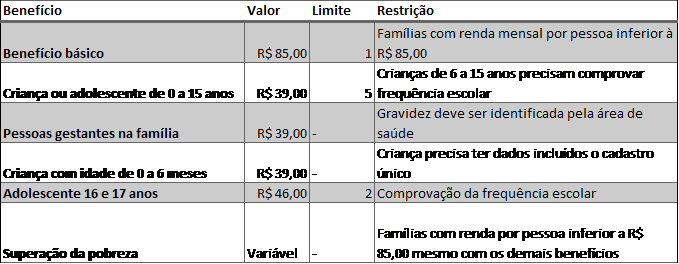
\includegraphics[width=1\textwidth]{beneficios_bolsa_familia.png}
\end{table} 

	É possível perceber que o Programa Bolsa Família desperta o interesse dos pesquisadores. Ao realizar busca nas bases de dados da ISI Web of Science, utilizando o argumento de pesquisa “Bolsa Família”, foram localizados mais de 150 artigos. A análise mais detalhada dessas publicações permite agrupá-las em três clusters a partir do tipo de análise realizada. O primeiro grupo é caracterizado por uma análise qualitativa dos impactos do Programa Bolsa Família. Autores como \cite{hall:2006}, \cite{fenwick:2009avoiding} e \cite{rocha2009developments} são alguns dos artigos que avaliam o sucesso do programa como política pública voltada para redução da pobreza. \cite{hall:2006} aparesenta o histórico do programa comparando com outros programas de transferência de renda, como o Fome Zero.  O segundo grupo definido, direcionou as pesquisas de forma mais quantitativa, buscando mensurar os impactos do programa bolsa família. \cite{glewwe2012impact} realizaram o cruzamento das bases de dados do Programa Bolsa Família com dados do censo escolar para mensurar o impacto do programa no número de matrículas, nas notas e no índice de desistência escolar. A partir da comparação dos dados de escolas com alunos cuja família recebia o benefício e escolas com alunos sem o benefício, as análises indicam que o Programa Bolsa Família elevou em mais de 5\% o número de alunos matriculados, reduziu em aproximadamente 0,5\% o índice de abandono escolar e elevou a nota média dos alunos.Outros estudos estão consolidados na Table 3


\begin{table}[ht]
\centering
\caption{Estudos quantitativos dos efeitos do Programa Bolsa Família \newline
Fonte: \cite{Rasella:2013}, \cite{glewwe2012impact}, \cite{Paes-Sousa:2011}, \cite{soares2010evaluating}} e \cite{Lignani:2011}
\label{tab:exTable3}
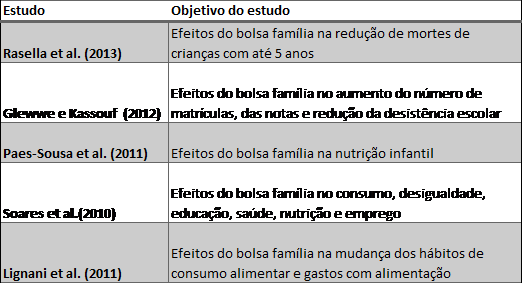
\includegraphics[width=1\textwidth]{bolsa_familia_semelhantes.png}
\end{table} 

	O terceiro grupo de artigos encontrado caracterizam-se por analisar os outros programas de transferência de renda brasileiros e mencionam em menor escala o Programa Bolsa Família. Pelo fato deste não ser o objeto principal do estudo, os artigos foram suprimidos da análise.



\section{Estatística}

In some conferences, the papers are published on CD-ROM while only the
abstract is published in the printed Proceedings. In this case, authors are
invited to prepare two final versions of the paper. One, complete, to be
published on the CD and the other, containing only the first page, with
abstract and ``resumo'' (for papers in Portuguese).

\section{Metodologia}

Section titles must be in boldface, 13pt, flush left. There should be an extra
12 pt of space before each title. Section numbering is optional. The first
paragraph of each section should not be indented, while the first lines of
subsequent paragraphs should be indented by 1.27 cm.

\section{Resultados}

The subsection titles must be in boldface, 12pt, flush left.

\section{Conclusões}
\label{sec:figs}

Figure and table captions should be centered if less than one line
(Figure~\ref{fig:exampleFig1}), otherwise justified and indented by 0.8cm on
both margins, as shown in Figure~\ref{fig:exampleFig2}. The caption font must
be Helvetica, 10 point, boldface, with 6 points of space before and after each
caption.

\begin{figure}[ht]
\centering
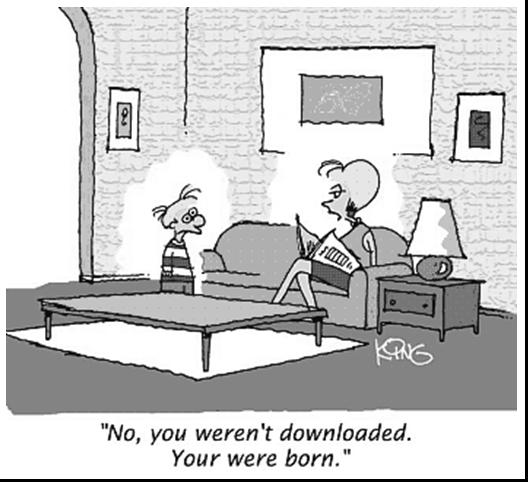
\includegraphics[width=.5\textwidth]{fig1.jpg}
\caption{A typical figure}
\label{fig:exampleFig1}
\end{figure}

\begin{figure}[ht]
\centering
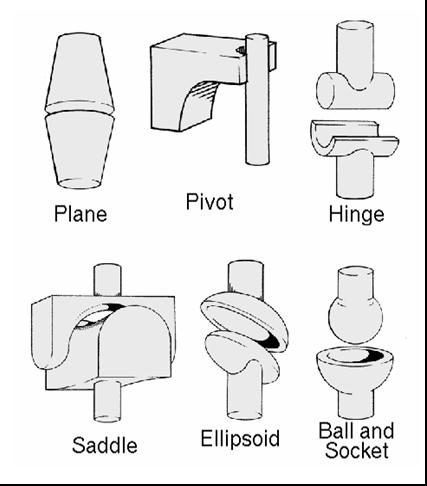
\includegraphics[width=.3\textwidth]{fig2.jpg}
\caption{This figure is an example of a figure caption taking more than one
  line and justified considering margins mentioned in Section~\ref{sec:figs}.}
\label{fig:exampleFig2}
\end{figure}

In tables, try to avoid the use of colored or shaded backgrounds, and avoid
thick, doubled, or unnecessary framing lines. When reporting empirical data,
do not use more decimal digits than warranted by their precision and
reproducibility. Table caption must be placed before the table (see Table 1)
and the font used must also be Helvetica, 10 point, boldface, with 6 points of
space before and after each caption.

\begin{table}[ht]
\centering
\caption{Variables to be considered on the evaluation of interaction
  techniques}
\label{tab:exTable8}
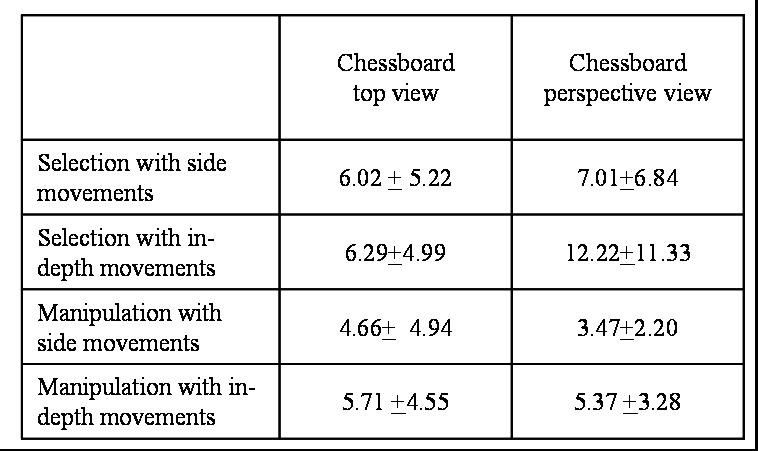
\includegraphics[width=.7\textwidth]{table.jpg}
\end{table}

\section{Images}

All images \cite{Angles:2010} and illustrations should be in black-and-white, or gray tones,
excepting for the papers that will be electronically available (on CD-ROMs,
internet, etc.). The image resolution on paper should be about 600 dpi for
black-and-white images, and 150-300 dpi for grayscale images.  Do not include
images with excessive resolution, as they may take hours to print, without any
visible difference in the result. 

\section{References}

Bibliographic references must be unambiguous and uniform.  We recommend giving
the author names references in brackets, e.g. \cite{Corbelini:2017},
\cite{Leavitt:2010}, and \cite{Stonebreaker:2010}.

The references must be listed using 12 point font size, with 6 points of space
before each reference. The first line of each reference should n not be
indented, while the subsequent should be indented by 0.5 cm.

\bibliographystyle{sbc}
\bibliography{sbc-template}

\end{document}
